        \chapter{Expected Outcome}
        \section{Desktop Outcome Expected}
        We've expected outcome in following scenario:\\
        Consider, a visually impaired people walking on a street using our system (Desktop App Active). S/he does not know what is going in front of her. But, can listen to voice. Suddenly, a car arrive in front of him. Now, Our system will detect the object that is appeared on camera module. Calculate distance. Then it will give a instruction something like. A car is at a distance 100m coming towards us with the speed of 10m/s. Be Alert, car will arrive within 10s.\\
        Also, Our System will detect any object (Used during training) in front like ditch, dogs, poll and alert people about the environment.\\
        The expected outcome for our Desktop App with GUI for the testing as well as debugging phase in starting of project is as follow:
        \begin{figure}[ht]
                \centering
                        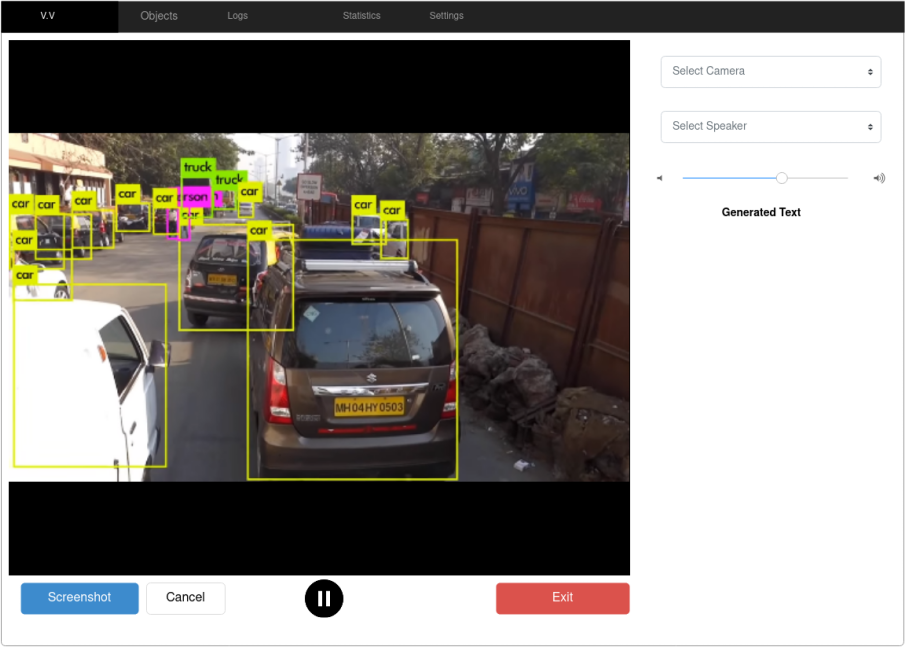
\includegraphics[width=0.9\textwidth]{img/VV1.png}
                        \caption{Mockup Design main window for desktop App}    
        \end{figure}
        \begin{figure}[ht]
                \centering
                        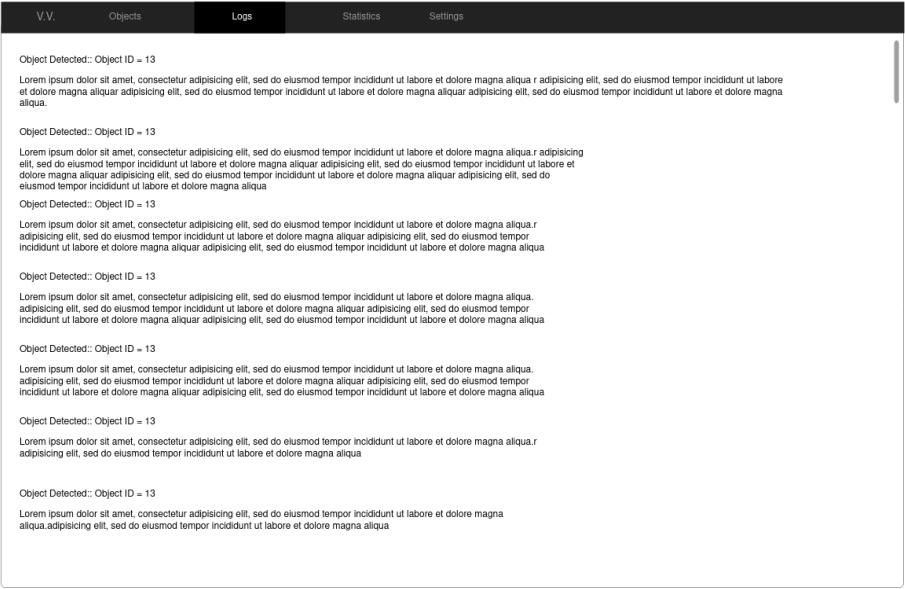
\includegraphics[width=0.77\textwidth]{img/VV2.png}
                        \caption{Mockup Design Logs window for desktop App}    
        \end{figure}
        \begin{figure}[ht]
                \centering
                        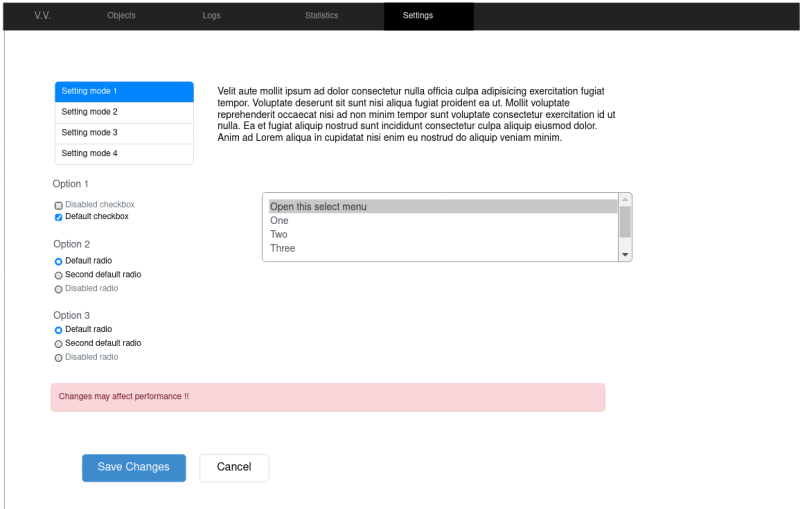
\includegraphics[width=0.77\textwidth]{img/VV3.png}
                        \caption{Mockup Design Settings window for desktop App}    
        \end{figure}\\
        As per our expectations in our desktop app we intended to develop good UI with smooth selection of desired objects to be detected which unfortunately proved to be inefficient interms of performance so the extra tabs were removed afterwards.
        Also with some logs and statistics tabs we thought of keeping each and every generated texts and detected objects throughout the program. 
        \pagebreak
        \section{Mobile Outcome Expected}
                \begin{figure}[h]
                        
\includegraphics[width=0.7\textwidth]{img/vv-mockup_720.png}
                \end{figure}